\chapter{Học sâu trên đồ thị}
\section{Từ bảng dữ liệu đến cấu trúc liên kết}
Trong dữ liệu bảng, mỗi hàng thường được xử lý bằng cùng một hàm dự đoán. Trong đồ thị, đặc trưng của một nút còn phụ thuộc vào những nút liên quan. Một bệnh, một xét nghiệm và một tài liệu có thể liên kết bằng các quan hệ khác nhau. Mạng nơ-ron đồ thị (GNN) học biểu diễn bằng cách trao đổi và tổng hợp thông tin dọc theo các cạnh. GNN được trình bày như một hướng học biểu diễn từ quan hệ. Hệ thống thực nghiệm trong báo cáo sử dụng truy vấn Neo4j; việc huấn luyện GNN nằm ngoài phạm vi thực nghiệm.

\subsection{Biểu diễn nút, cạnh và đặc trưng}
Đặt đồ thị $G=(V,E)$ với $n$ nút, ma trận đặc trưng $X\in\mathbb{R}^{n\times d}$ và ma trận kề $A$. Với đồ thị có hướng, $A_{ij}$ và $A_{ji}$ có thể khác nhau. Với đồ thị tri thức, một cạnh còn mang loại quan hệ và nguồn bằng chứng. Nếu bỏ các thuộc tính này để tạo đồ thị vô hướng, ta đã thay đổi ý nghĩa dữ liệu; phép chuyển đổi phải được công bố trong thiết kế thí nghiệm.
\section{Cơ chế truyền thông điệp}
\subsection{Tổng hợp thông tin lân cận}
Một tầng truyền thông điệp có thể viết dưới dạng:
\[
m_v^{(l)}=\operatorname{AGG}_{u\in\mathcal{N}(v)} M_l(h_v^{(l)},h_u^{(l)},e_{uv}),\qquad
h_v^{(l+1)}=U_l(h_v^{(l)},m_v^{(l)}).
\]
Hàm tổng hợp phải không phụ thuộc thứ tự liệt kê các nút láng giềng. Tổng, trung bình và cực đại là các lựa chọn thông dụng. Hàm cập nhật kết hợp thông tin của chính nút với thông tin từ láng giềng. Sau hai tầng, một nút có thể nhận thông tin từ vùng lân cận hai bước, nhưng điều đó không đồng nghĩa với suy luận logic hai bước có bảo đảm.

\subsection{Chuẩn hóa và cập nhật biểu diễn trong GCN}
Trong một GCN, thêm cạnh tự nối rồi chuẩn hóa theo bậc:
\[
\widetilde A=A+I,\quad \widetilde D_{ii}=\sum_j\widetilde A_{ij},\qquad
H^{(l+1)}=\sigma(\widetilde D^{-1/2}\widetilde A\widetilde D^{-1/2}H^{(l)}W^{(l)}).
\]
Ma trận $W^{(l)}$ được học từ hàm mất mát. Chuẩn hóa giúp hạn chế việc nút bậc cao đóng góp tổng thông tin lớn chỉ vì có nhiều cạnh. Đối với bài toán phân loại nút, mất mát chỉ tính trên các nút có nhãn thuộc tập huấn luyện. Việc dùng cấu trúc của nút test trong quá trình truyền thông điệp cần được ghi rõ là thiết lập transductive.
\section{Các biến thể và lựa chọn phù hợp}
\subsection{GraphSAGE, GAT và R-GCN}
GraphSAGE lấy mẫu láng giềng và học hàm tổng hợp, phù hợp khi cần xử lý các nút mới có đặc trưng. GAT học trọng số chú ý giữa các nút liên quan, nhưng hệ số chú ý không tự trở thành lời giải thích nhân quả. Với đồ thị nhiều loại quan hệ, R-GCN dùng các phép biến đổi phụ thuộc loại cạnh. Kiến trúc được lựa chọn dựa trên loại quan hệ, quy mô đồ thị và nhiệm vụ đánh giá.

\subsection{Nhiệm vụ học trên đồ thị}
Ba đầu ra thường gặp là nhãn nút, khả năng tồn tại cạnh và nhãn toàn đồ thị. Các đầu ra này khác với câu trả lời của chatbot. GNN có thể giúp truy xuất hoặc xếp hạng bằng chứng, còn phần diễn đạt vẫn cần một cơ chế tạo phản hồi và kiểm tra nguồn. Nếu dự đoán một cạnh chưa có trong KB, hệ thống phải đánh dấu đó là giả thuyết của mô hình, không tự thêm như một sự thật đã kiểm chứng.
\section{Liên hệ với kho tri thức của hệ thống}
Kho đang chạy có 60 nút Concept và 32 cạnh RELATED\_TO. Tên quan hệ thật nằm ở thuộc tính label, mã tài liệu ở document. Ví dụ, khái niệm HbA1c nối với đường huyết trung bình bằng quan hệ phản ánh. Có thể tạo một ma trận kề từ các cặp này và vector đặc trưng từ văn bản, nhưng kho nhỏ và thiếu nhãn nhiệm vụ khiến việc huấn luyện một GNN chưa có cơ sở đánh giá đáng tin cậy.

Vì vậy bản triển khai giữ cách tra cứu có nguồn: tìm đoạn văn phù hợp rồi lấy các cạnh cùng mã tài liệu. Điểm mạnh là mỗi quan hệ đều kiểm tra được. Điểm yếu là hệ thống chưa học biểu diễn liên kết và chưa suy luận trên các quan hệ thiếu. Do chưa có nhãn phục vụ đánh giá GNN, thực nghiệm tập trung vào khả năng truy xuất và kiểm tra nguồn của các quan hệ.
\section{Thiết kế một thí nghiệm mở rộng}
\subsection{Dự đoán liên kết}
Nếu mở rộng, cần xây dựng nhãn và quy trình kiểm chứng trước. Với dự đoán liên kết, tách các cạnh test trước khi tạo đặc trưng, kiểm soát cạnh đảo và các quan hệ trùng nghĩa. Mẫu âm phải phù hợp miền, vì một cạnh chưa được ghi nhận không nhất thiết là cạnh sai. So sánh với các đường cơ sở như tương đồng văn bản và số láng giềng chung trên cùng phép chia.

\subsection{Phân loại nút và tiêu chí đánh giá}
Với phân loại nút, ghi rõ số nút train, validation và test, cách tạo đặc trưng và liệu test có tham gia cấu trúc đồ thị hay không. Báo cáo macro-F1, kết quả nhiều seed và thời gian chạy. Không dùng kết quả phân loại nút của một đồ thị trích dẫn để kết luận hiệu quả tư vấn y tế.
\section{Hạn chế cần kiểm soát}
Quá nhiều tầng có thể làm biểu diễn các nút gần nhau trở nên khó phân biệt. Nút trung tâm có thể tập trung nhiều thông tin, còn lỗi liên kết làm lan truyền tín hiệu sai. Một KB có nguồn yếu vẫn tạo ra đầu vào yếu cho GNN. Cần kiểm soát nguồn, loại quan hệ và phiên bản dữ liệu trước khi tối ưu kiến trúc.
\chapter{Agent, hệ đa agent và học tăng cường}
\section{Khái niệm agent}
\subsection{Thành phần và phạm vi hoạt động}
Agent nhận quan sát, duy trì trạng thái phục vụ nhiệm vụ và lựa chọn hành động trong một môi trường. Một hàm dự đoán chỉ ánh xạ đầu vào sang nhãn; một agent còn cần xác định khi nào gọi hàm đó, xử lý trường hợp thiếu dữ liệu và chuyển kết quả cho thành phần khác. Mức tự chủ phụ thuộc vào phạm vi hành động được trao và cơ chế phản hồi.

\subsection{Biểu diễn agent trong chương trình}
Trong project, agent là các đối tượng phần mềm với tên, bộ xử lý thông điệp và bộ nhớ cục bộ cho lượt xử lý. MessageBus định tuyến REQUEST tới đúng handler và ghi INFORM hoặc FAILURE khi hoàn tất. Việc triển khai trong một tiến trình giúp tái lập dễ hơn, nhưng không cung cấp tính độc lập triển khai của một hệ phân tán.
\section{Phối hợp và giao thức}
\subsection{Tổ chức điều phối}
Điều phối tập trung giúp xác định thứ tự xử lý và hạn chế gọi công cụ không cần thiết. Truy xuất và mô hình có chức năng khác nhau: một bên trả bằng chứng, bên kia trả kết quả tính toán. Agent đối chiếu kiểm tra phạm vi diễn giải; agent phản hồi tổng hợp nội dung. Kết quả của hai nhánh đều đi đến đầu ra trợ giúp theo sơ đồ trên bảng.

\subsection{Thông điệp và xử lý thất bại}
Một giao thức tối thiểu cần xác định người gửi, người nhận, loại thông điệp, nội dung và điều kiện thất bại. Phiên bản hiện có bốn trường này, cộng nhật ký tuần tự theo từng yêu cầu. Khi mở rộng cần thêm mã hội thoại, mã yêu cầu, hạn xử lý và cơ chế chống xử lý lặp. Không nên đánh đồng việc ghi một dòng log với việc một agent đã thực thi: handler phải thật sự nhận yêu cầu và tạo kết quả.
\section{Mô hình học tăng cường}
\subsection{Trạng thái, hành động và phần thưởng}
Một quá trình quyết định Markov được mô tả bởi trạng thái, hành động, động lực chuyển trạng thái, phần thưởng và hệ số chiết khấu. Mục tiêu là tối đa hóa tổng phần thưởng kỳ vọng. Trong Q-learning dạng bảng:
\[
Q(s,a)\leftarrow Q(s,a)+\alpha\left[r+\gamma\max_{a'}Q(s',a')-Q(s,a)\right].
\]
\subsection{Khám phá và khai thác}
Hành động khám phá giúp quan sát các lựa chọn chưa biết; khai thác chọn giá trị hiện cao nhất. Cần tách đánh giá khỏi huấn luyện, cố định seed khi tái lập và tránh đánh giá chỉ trên các episode có khám phá nếu mục tiêu là đo chính sách cuối cùng.
\section{Kết hợp học với luật}
\subsection{Điều kiện hợp lệ của hành động}
Luật biểu diễn những điều kiện phải kiểm tra trực tiếp, chẳng hạn chưa đủ trường thì chưa suy luận, không có tài liệu thì không khẳng định đã có bằng chứng. Chính sách học chỉ lựa chọn trong phạm vi cho phép. Cách kết hợp này có thể viết là chọn hành động tốt nhất trên tập hành động hợp lệ $\mathcal A_{safe}(s)$, hoặc kiểm tra và thay thế hành động sau khi đề xuất.

\subsection{Chính sách trong môi trường một bước}
Bản demo dùng môi trường một bước với bốn trạng thái và ba hành động. Do episode kết thúc ngay, biểu thức cập nhật chỉ còn $Q\leftarrow Q+\alpha(r-Q)$. Đây là minh họa học chính sách điều phối, không phải agent tự học điều trị. Phần thưởng được thiết kế thủ công nên kết quả tốt chỉ chứng minh chính sách đã học được quy tắc của môi trường mô phỏng.
\section{Tích hợp mô hình và tri thức}
Các mô hình học máy và học sâu cung cấp công cụ tính toán; đồ thị tri thức cung cấp bằng chứng có cấu trúc; truy xuất chọn thông tin theo yêu cầu. Hệ đa agent kết nối các công cụ đó thành quy trình phục vụ người dùng. Đóng góp mới của project nằm ở việc tích hợp hai nhánh, lưu dấu vết thực thi, đưa dữ liệu lên Neo4j và tạo giao diện trình diễn có thể kiểm tra.

\section{Sản phẩm tích hợp và kết quả triển khai}
GlucoGuide kết nối hai mô hình MLP, bộ truy xuất văn bản và cơ sở dữ liệu Neo4j trong cùng một ứng dụng. Người dùng có thể hỏi kiến thức, đọc căn cứ và chuyển kết quả thực nghiệm sang hội thoại. Hình dưới minh họa giao diện của hệ thống; quy trình kiểm thử được trình bày ở phần II.
\productlink{Ứng dụng GlucoGuide}{https://dirt-lucky-capture-mighty.trycloudflare.com}
\begin{figure}[!htbp]\centering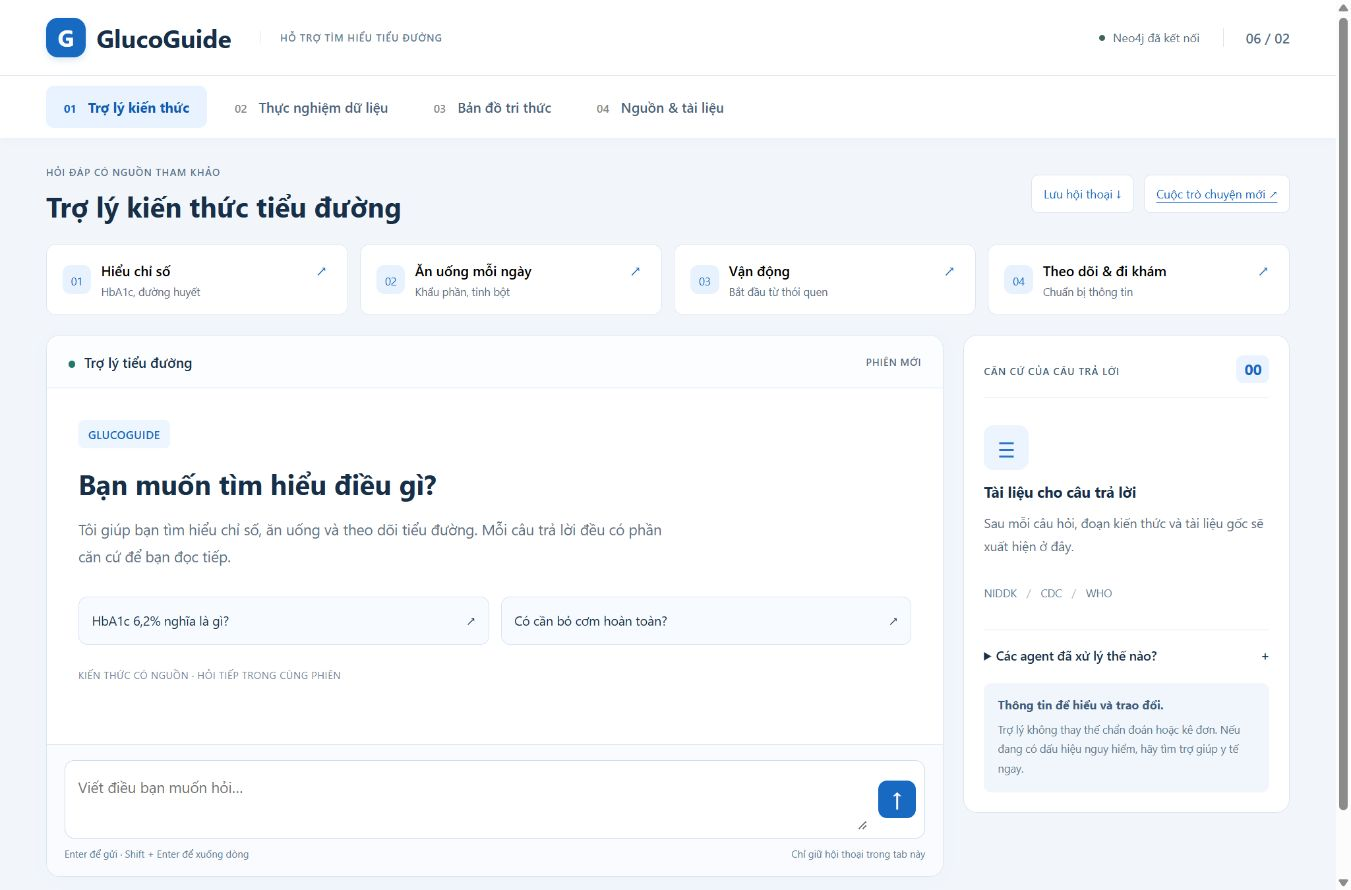
\includegraphics[width=\linewidth]{demo-home.png}\caption{Giao diện sản phẩm tích hợp mô hình, tri thức và hội thoại.}\end{figure}
